\documentclass[conference]{IEEEtran}
\IEEEoverridecommandlockouts
% The preceding line is only needed to identify funding in the first footnote. If that is unneeded, please comment it out.
\usepackage{cite}
\usepackage{amsmath,amssymb,amsfonts}
\usepackage{algorithmic}
\usepackage{graphicx}
\usepackage{textcomp}
\usepackage{xcolor}
\usepackage{multirow}
\usepackage{rotating}
\usepackage{mdframed}
\usepackage{hyperref}
\usepackage{tikz}
\usepackage{makecell}
\usepackage{tcolorbox}
\usepackage{amsthm}
\usepackage{tabularx}
\usepackage{array}
\usepackage{float}
\usepackage{placeins}
\usepackage[T1]{fontenc}


%\usepackage[english]{babel}
\usepackage{pifont} % checkmarks
%\theoremstyle{definition}
%\newtheorem{definition}{Definition}[section]


\usepackage{listings}
\lstset
{ 
    basicstyle=\footnotesize,
    numbers=left,
    stepnumber=1,
    xleftmargin=5.0ex,
}

%SCJ
\usepackage{subcaption}
\usepackage{array, multirow}
\usepackage{enumitem}

\def\BibTeX{{\rm B\kern-.05em{\sc i\kern-.025em b}\kern-.08em
    T\kern-.1667em\lower.7ex\hbox{E}\kern-.125emX}}
\begin{document}
      
\title{Smart Greenhouse Farming}

\author{
    \IEEEauthorblockN{
        Jacob Høck Michelsen\IEEEauthorrefmark{1},
        Shad Bin Bari\IEEEauthorrefmark{1},
        Md Mannan Miah\IEEEauthorrefmark{1},
        Faiza Akter\IEEEauthorrefmark{1}
    }
    \IEEEauthorblockA{
        University of Southern Denmark, SDU Software Engineering, Odense, Denmark\\
        Email: \IEEEauthorrefmark{1}\texttt{\{jacmi13@student.sdu.dk, shbin25@student.sdu.dk, mmiah25@student.sdu.dk, faakt25@student.sdu.dk\}}
    }
}
\maketitle
\begin{abstract}
The rising demand for effective and sustainable farming has led to the emergence of smart farming technology.
This project provides a Smart Farming Software Platform that is utilized to automate and monitor greenhouses in a scalable and secure software architecture.
Focusing exclusively on the software layer, the system enables real-time monitoring of soil moisture, temperature, humidity, and light of multiple greenhouse factories.
With a microservices-based, event-driven architecture, sensor data are processed and saved continuously, allowing for automatic control action such as watering or heating upon reaching to threshold values.
There is also a specialized dashboard providing administrators with real-time insight into the state of each greenhouse, as well as a sensor simulator allowing for testing and validation without hardware.
Quality attributes addressed under the key ones are availability, scalability, fault tolerance, and security, which renders the platform 24/7 deployable in production.
Overall, the system described in this work demonstrates how software architecture may be placed center stage to enable future sustainable, automated, and data-driven agriculture.
\end{abstract}

\begin{IEEEkeywords}
Smart Greenhouse farming, automated irrigation, event driven system, real time monitoring, sustainable agriculture
\end{IEEEkeywords}

\section{Introduction and Motivation}
%Introduction and motivate the problem
In modern agriculture there is a strong pressure to produce more food with less resources. Greenhouse production especially depends on careful control of soil moisture, temperature and humidity to keep plants healthy and to avoid wasting water and energy. Many smaller greenhouses still rely on simple timers or local controllers, and a lot of decisions are done manually. This makes it hard to monitor many greenhouses at once and to react quickly when something goes wrong.

At the same time, cheap sensors, IoT devices and cloud technologies make it possible to collect and process data from many greenhouses in real time. However, it is not enough to just “connect everything to the cloud”. The software architecture behind such a platform has a big impact on qualities like performance, scalability, availability and safety. Software architecture is the set of structures of a system, including elements, their relations and their properties, that we use to reason about the system. If we do not think about architecture early, we risk ending up with a system that is difficult to change, hard to scale and almost impossible to verify.

In this project we focus on designing and analysing the architecture for a Smart Farming Software Platform for monitoring and controlling multiple greenhouses. We follow the ideas from the ASAAT course: document architectural requirements, design the architecture in a systematic way, and then use both formal verification and experiments to evaluate if the architecture really supports the required quality attributes.

\section{Problem and Approach}
The main problem we address is how to design a reliable and scalable software architecture for a smart greenhouse platform that:

\label{sec:problem}
\emph{Problem.}
\begin{enumerate}
    \item continuously receives sensor data (e.g. soil moisture),
    \item decides when to start or stop watering,
    \item updates a dashboard for operators,
    \item and at the same time supports important quality attributes like availability, performance, modifiability and safety.
\end{enumerate}

Concretely, the system should be able to handle many greenhouses and frequent sensor events, keep working even when some components fail temporarily (e.g. message broker or database issues), and be structured in a way that we can analyse and evolve it over time.


\subsection{Research questions}

\begin{enumerate}
    \item  How can we design a microservice-based, event-driven architecture for smart greenhouse control that supports key quality attributes such as availability, scalability and modifiability?

    \item How can the system architecture facilitate low-latency, real-time propagation of sensor events to a dashboard in a distributed smart farming configuration?
\end{enumerate}

\subsection{Approach.}
The following steps are taken to answer this paper's research questions: 
\begin{enumerate}
    \item Requirements and quality attributes: We derive functional requirements from the smart greenhouse scenario and then express key quality attributes (availability, performance, modifiability, safety, integrability) as quality attribute scenarios in the Len Bass format.

    \item Design, modelling and analysis: We design a microservice-based architecture with RabbitMQ as a message bus and a shared database. We create design-level architecture diagrams and link architectural decisions to tactics and patterns (e.g. message bus, microservices, layering, containerisation, wrappers).

    \item Prototype implementation: We implement the architecture using multiple services (SimulatorUI, GreenhouseFactoryService, SoilMoistureService, WaterService, Dashboard), a RabbitMQ message bus, a database, and containerisation. This directly maps to the “Source Code” criterion in the rubric: message bus, DB, Docker, and V\&V artefacts.

    \item Empirical evaluation: 
    \begin{itemize}
        \item Design a software experiment where we increase the number of simulated greenhouses and measure throughput and failure rates for fixed time windows, in line with the empirical evaluation guidance from the course.
        
        \item  Optionally measure simple end-to-end latency from sensor event to dashboard update, or at least discuss how the current architecture supports low-latency propagation .
    \end{itemize}
    

   

\end{enumerate}



\section{Related work}
\label{sec:related_work}
Our work is related to architectures for smart factories and reconfigurable production systems, where the main goals are flexibility, integration and cost-effective operation.\\

Wan (2019) proposes a reconfigurable smart factory for drug packing with a clear three-layer architecture: a perception layer for data collection, a deployment layer for decision and control logic, and an execution layer where physical devices operate. This structure separates low-level sensing/actuation from higher-level orchestration and makes it easier to reconfigure the system for different products or packaging tasks. We follow a similar idea in our smart farming platform by separating sensor collection, processing/decisions and presentation, although our implementation is based on microservices and RabbitMQ instead of the exact layers used in the drug packing factory.\\

Yazen Alsafi (2010) presents an ontology-based reconfiguration agent for intelligent mechatronic systems.  In that work, the agent uses ontological knowledge about the manufacturing environment to decide how to reconfigure modular systems without human intervention. The focus is on semantic information (what capabilities components have and how they can be combined) and on autonomous reconfiguration. While our system does not include an ontology or a full agent framework, the idea of having explicit knowledge about system elements and using that knowledge to drive reconfiguration is similar to how we think about adding or changing greenhouses in our architecture.\\

Several authors focus on reconfigurable production control systems. Leitão and co-authors describe architectures for smart and heterogeneous production components and show how agent-based and service-oriented principles can be combined to support flexible and evolvable production systems. Angione and others also study reconfigurable production control with an emphasis on architectures that can be adapted when the production process or product mix changes. These works highlight that architectural decisions (e.g. holonic or multi-agent control, service-orientation) strongly influence how easy it is to reconfigure a system during its life cycle. Our smart farming system faces a similar challenge when we want to add new greenhouses, new types of sensors, or new control logic without redesigning everything.\\


The concept of Reconfigurable Manufacturing Systems (RMS), introduced by Koren and colleagues, provides a broader background. In their classic work, they argue that manufacturing systems must be able to quickly change structure and capacity in a cost-effective way to respond to market changes.  RMSs combine some of the flexibility of flexible manufacturing systems with the efficiency of dedicated lines. Bortolini et al. (2018) provide a literature review and research trends on RMSs, and emphasise design principles such as modularity, scalability and reconfigurability as key for modern production systems. \\


In our project we do not design a full RMS, but the same principles apply: we want an architecture that can be scaled (more greenhouses, more data), reconfigured (new services, new quality attributes) and still remain cost-effective and understandable.\\

Compared to these works, our contribution is more focused on the software architecture and analysis side for a specific smart farming case. We:

\begin{itemize}
    \item take inspiration from three-layer and agent-based architectures (Wan; Alsafi) for structuring the system,
    \item adopt reconfigurability and cost-effectiveness as guiding principles from RMS literature (Koren; Bortolini),
    \item and combine this with the ASAAT toolbox: explicit quality attribute scenarios, microservice and message-bus design, formal verification using timed automata, and an empirical evaluation of the implemented prototype
\end{itemize}



\section{Use Case}
\label{sec:use_case}
\FloatBarrier

\begin{table}[h]
\centering
\caption{Use case \#1: View greenhouse data}
\resizebox{\columnwidth}{!}{
\begin{tabular}{|l|p{5cm}|} \hline
Use case & View greenhouse data \\ \hline
Actors & Administrator \\ \hline
Preconditions & At least one greenhouse factory and greenhouse exist. \\ \hline
Steps &
\begin{enumerate}
\item Administrator opens the dashboard.
\item Dashboard displays whether watering is on or off.
\end{enumerate} \\ \hline
Postconditions & Administrator can view real-time water status. \\ \hline
Related QAS & \#2, \#3, \#4 \\ \hline
\end{tabular}}
\end{table}

\begin{table}[!t]
\centering
\caption{Use case \#2: Simulate greenhouse sensors}
\resizebox{\columnwidth}{!}{
\begin{tabular}{|l|p{5cm}|} \hline
Use case & Simulate greenhouse sensors \\ \hline
Actors & User simulating sensor events \\ \hline
Preconditions &
\begin{itemize}
\item Greenhouse factory exists
\item Simulator supports SoilMoistureEvent and WaterEvent
\end{itemize} \\ \hline
Steps &
\begin{enumerate}
\item User opens simulator UI
\item Enters factory and greenhouse ID
\item Triggers SoilMoistureEvent
\item Event published to message bus
\item Services process event
\item Dashboard updates in real time
\end{enumerate} \\ \hline
Postconditions & Simulated events behave like real sensor data \\ \hline
Related QAS & \#1 \\ \hline
\end{tabular}}
\end{table}

\begin{table}[!t]
\centering
\caption{Use case \#3: Automatic watering}
\resizebox{\columnwidth}{!}{
\begin{tabular}{|l|p{5cm}|} \hline
Use case & Automatic watering based on soil moisture \\ \hline
Actors & SoilMoistureService, WaterService \\ \hline
Preconditions &
\begin{itemize}
\item Soil moisture sensors configured
\item Threshold value defined
\end{itemize} \\ \hline
Steps &
\begin{enumerate}
\item Sensor detects low moisture
\item SoilMoistureService publishes WaterEvent
\item WaterService turns water on/off
\item Status stored and dashboard updated
\end{enumerate} \\ \hline
Postconditions & Plants are watered automatically \\ \hline
Related QAS & \#4 \\ \hline
\end{tabular}}
\end{table}



\FloatBarrier


\section{Quality Attribute Scenario}
\label{sec:qas}
\FloatBarrier
To specify quality attribute requirements and scenarios we use the following definition and  structure \cite{bass2013}

\begin{table}[h]
    \centering
    \caption{Quality Attribute Scenario}
    \begin{tabular}{|l|p{4cm}|} \hline
        Source of stimulus & This is some entity that generated the stimulus  \\ \hline
        
        Stimulus & The stimulus is a condition that requires a response when it arrives at a system\\ \hline
        
        Environment & The stimulus occurs under certain conditions.\\ \hline
        
        Artifact  & Some artifact is stimulated\\ \hline

        Response  & The response is the activity undertaken as the result of an arrival of the stimulus\\ \hline

        Response measure & When the response occurs, it should be measurable in some fashion so that the requirement can be tested \\
        \hline
    \end{tabular}
    
    \label{tab:placeholder}
\end{table}


We have defined the following quality attribute scenarios for the system.

\begin{table}[!t]
\centering
\caption{Quality Attribute Scenarios for the Smart Farming Platform}
\renewcommand{\arraystretch}{1.15}
\resizebox{\columnwidth}{!}{
\begin{tabular}{|l|p{7.5cm}|}
\hline
\textbf{Scenario} & \textbf{Description} \\ \hline

High message load handling &
\textbf{Source:} Greenhouses sending data;\\ &
\textbf{Stimulus:} High event volume overloads the message bus;\\ &
\textbf{Environment:} Normal operation;\\ &
\textbf{Artifact:} Message bus and microservices;\\ &
\textbf{Response:} Events are queued and processed;\\ &
\textbf{Response Measure:} $\geq$ 99\% throughput;\\ &
\textbf{Related Tactic:} Message queuing. \\ \hline

Database unavailability &
\textbf{Source:} Network error;\\ &
\textbf{Stimulus:} Database becomes unavailable;\\ &
\textbf{Environment:} Error condition;\\ &
\textbf{Artifact:} Greenhouse Factory service;\\ &
\textbf{Response:} Retry until recovery;\\ &
\textbf{Response Measure:} Data stored if recovery occurs within 1 minute;\\ &
\textbf{Related Tactic:} Retry mechanism. \\ \hline

Invalid sensor data &
\textbf{Source:} Sensor device;\\ &
\textbf{Stimulus:} Invalid factory or greenhouse ID;\\ &
\textbf{Environment:} Normal operation;\\ &
\textbf{Artifact:} Greenhouse Factory service;\\ &
\textbf{Response:} Input validation and rejection;\\ &
\textbf{Response Measure:} Fault detected within $<$1 second;\\ &
\textbf{Related Tactic:} Validation and fault detection. \\ \hline

System update deployment &
\textbf{Source:} Developers;\\ &
\textbf{Stimulus:} New version deployment;\\ &
\textbf{Environment:} Normal operation;\\ &
\textbf{Artifact:} Containers;\\ &
\textbf{Response:} Rolling update;\\ &
\textbf{Response Measure:} Zero downtime;\\ &
\textbf{Related Tactic:} Containerization and rolling updates. \\ \hline

\end{tabular}
}

\label{tab:qas_ieee}
\end{table}

\FloatBarrier

\section{Design and Analysis Modelling}
\label{sec:design_and_analysis_modelling}

To achieve the goals specified by the quality attribute scenarios the system could implement the following tactics \footnote{Lecture 2: Software Architecture Recap, SDU, slide 7.}  

\begin{table}[h]
\centering
\caption{Architecture Tactics and Design Decisions}
\renewcommand{\arraystretch}{1.15}
\resizebox{\columnwidth}{!}{
\begin{tabular}{|l|p{7.5cm}|}
\hline
\textbf{Tactic Group} & \textbf{Description} \\ \hline

Performance &
\textbf{Tactic:} Control resource demand \\
& \textbf{Supported:} Yes \\
& \textbf{Risk:} Low \\
& \textbf{Design Decision:} RabbitMQ is used to handle input events between microservices \\
& \textbf{Rationale:} Ensures high throughput and prevents overload \\ \hline

Availability &
\textbf{Tactic:} Recover from fault (Retry) \\
& \textbf{Supported:} Yes \\
& \textbf{Risk:} Medium \\
& \textbf{Design Decision:} Retry policies added in microservices \\
& \textbf{Rationale:} Keeps the system running if the database or message bus is temporarily unavailable \\ \hline

Modifiability &
\textbf{Tactic:} Reduce module size, increase cohesion \\
& \textbf{Supported:} Yes \\
& \textbf{Risk:} Medium \\
& \textbf{Design Decision:} Separate microservices (SimulatorUI, GreenhouseFactoryService, SoilMoistureService, WaterService, Dashboard) \\
& \textbf{Rationale:} Enables independent deployment and reduces coupling, at the cost of increased deployment complexity \\ \hline

Deployability &
\textbf{Tactic:} Continuous deployment support \\
& \textbf{Supported:} Yes \\
& \textbf{Risk:} Medium \\
& \textbf{Design Decision:} Docker containers deployed using Kubernetes \\
& \textbf{Rationale:} Enables 24/7 production availability while rolling updates occur \\ \hline

\end{tabular}
}

\label{tab:tactics_ieee}
\end{table}

\subsection{Trade-Offs}

In the following table trade-offs are described for the chosen tactics.

\begin{table}[h]
\centering
\caption{Trade-offs for the Chosen Architecture Tactics}
\renewcommand{\arraystretch}{1.15}
\resizebox{\columnwidth}{!}{
\begin{tabular}{|l|p{7.5cm}|}
\hline
\textbf{Trade-off} & \textbf{Description} \\ \hline

RabbitMQ usage &
\textbf{Quality Attributes Impacted:} Performance, Scalability \\
& \textbf{Trade-off:} Improves performance and service decoupling but increases configuration effort, monitoring overhead, and introduces asynchronous behavior complexity \\
& \textbf{Risk:} Medium \\
& \textbf{Related Tactic:} \#1 \\ \hline

Retry policies &
\textbf{Quality Attributes Impacted:} Availability, Reliability \\
& \textbf{Trade-off:} Improves availability but may mask failures or cause cascading retries if not combined with backoff or circuit breakers \\
& \textbf{Risk:} Medium \\
& \textbf{Related Tactic:} \#2 \\ \hline

Microservices architecture &
\textbf{Quality Attributes Impacted:} Modifiability, Maintainability \\
& \textbf{Trade-off:} Increases modifiability and independent deployment, but adds operational complexity and distributed system challenges \\
& \textbf{Risk:} Medium \\
& \textbf{Related Tactic:} \#3 \\ \hline

CI/CD with rolling updates &
\textbf{Quality Attributes Impacted:} Deployability, Availability \\
& \textbf{Trade-off:} Improves uptime and deployability, but requires expertise and orchestration infrastructure such as Kubernetes \\
& \textbf{Risk:} Medium \\
& \textbf{Related Tactic:} \#4 \\ \hline

\end{tabular}
}

\label{tab:tradeoffs_ieee}
\end{table}

\begin{figure}[!t]
  \centering
  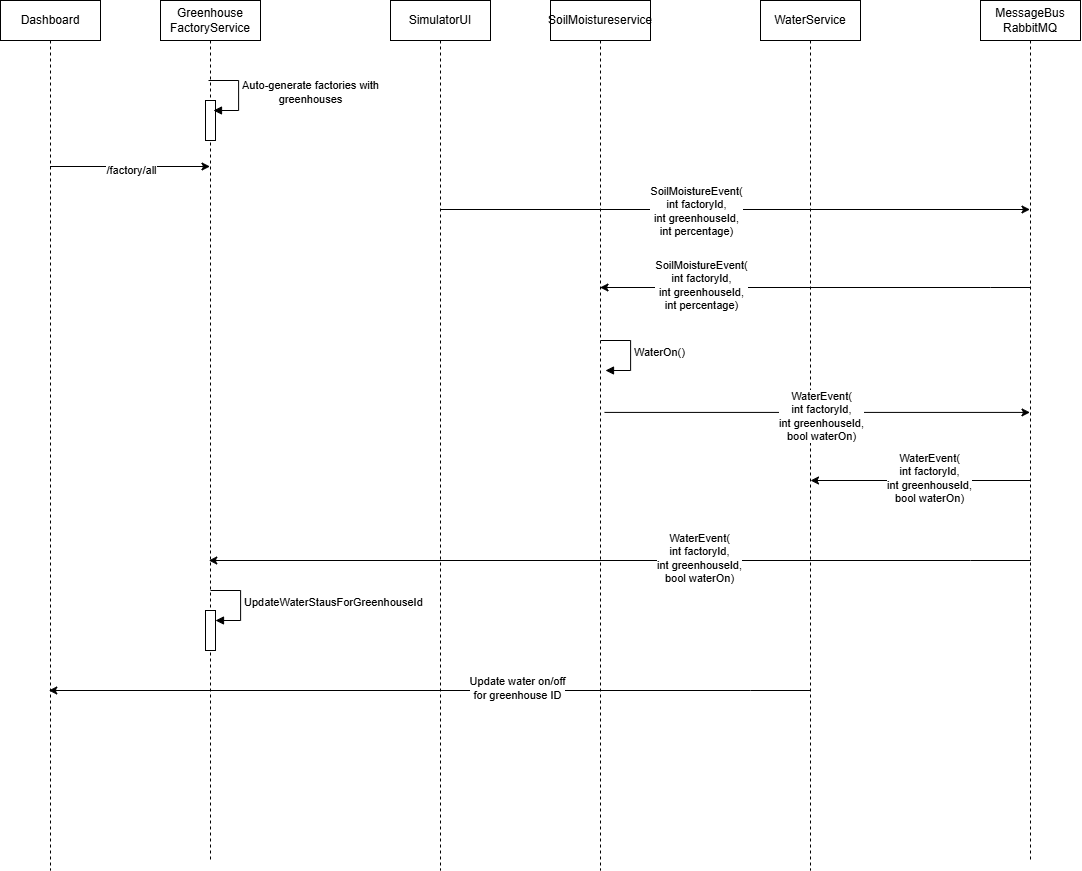
\includegraphics[width=85mm]{SequenceDiagram.drawio.png}
  \caption{Sequence Diagram}
  \label{fig:package diagram}
\end{figure}

In the above sequence diagram the flow between the micro services is illustrated.

\FloatBarrier


 \begin{table}[h]
    \centering
    \caption{Quality Attribute Scenario}
    \begin{tabular}{|l|p{4cm}|} \hline
        Service & Descriptions  \\ \hline
        
        SimulatorUI & Build as an event simulator instead of a real greenhouse sending data\\ \hline
        
        MessageBus & Used as async communication between micro services.\\ \hline
        
        SoilMoistureService  & Microservice responsible for calculating whether a greenhouse needs to turn on water or not\\ \hline

        WaterService  & Microservice responsible for live-update Dashboard if water is on for the greenhouse or not\\ \hline

        GreenhouseFactoryService & Microservice responsible for creating factories and greenhouses and persistent it in a database if water is on or not for a greenhouse \\
        \hline

        Dashboard & Microservice UI responsible for displaying factories and greenhouses and show the administrator or operator if the water is on for the specific greenhouse.\\ \hline
    \end{tabular}
    
    \label{tab:placeholder}
\end{table}


\FloatBarrier
In the above deployment diagram the applications are illustrated with technology stack, running port and communication type.


\begin{figure}[!t]
  \centering
  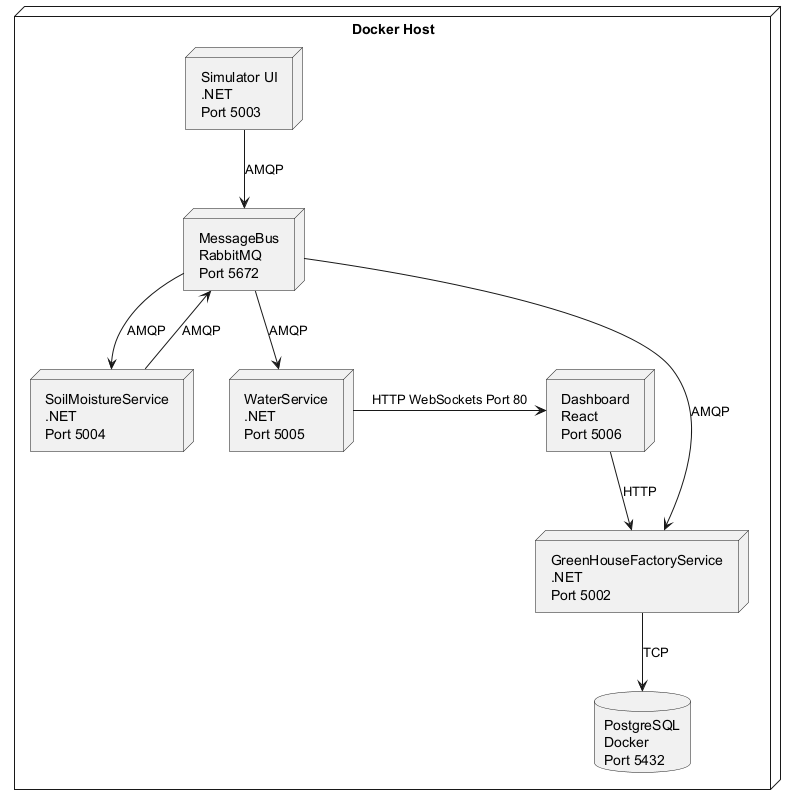
\includegraphics[width=85mm]{deployment diagram.png}
  \caption{Deployment Diagram }
  \label{fig:deployment diagram}
\end{figure}
\FloatBarrier

\clearpage
In the following package diagram the packages are shown within  SoilMoistureService which follows the clean architecture model.

\FloatBarrier
\begin{figure}[htbp]
  \centering
  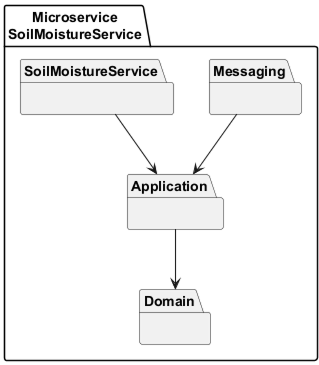
\includegraphics[width=85mm]{package diagram.png}
  \caption{Package Diagram }
  \label{fig:package diagram}
\end{figure}


\FloatBarrier
\section{Formal verification and validation}
\label{sec:formal_v_and_v}

The suggested smart farming system architecture is formally verified and validated in this part using UPPAAL, a tool for simulating, modelling, and verifying real-time systems based on timed automata. This analysis's objective is to confirm that, regardless of implementation specifics, the system satisfies its essential functional and temporal criteria under all potential execution circumstances.

\begin{figure}[htbp]
  \centering
  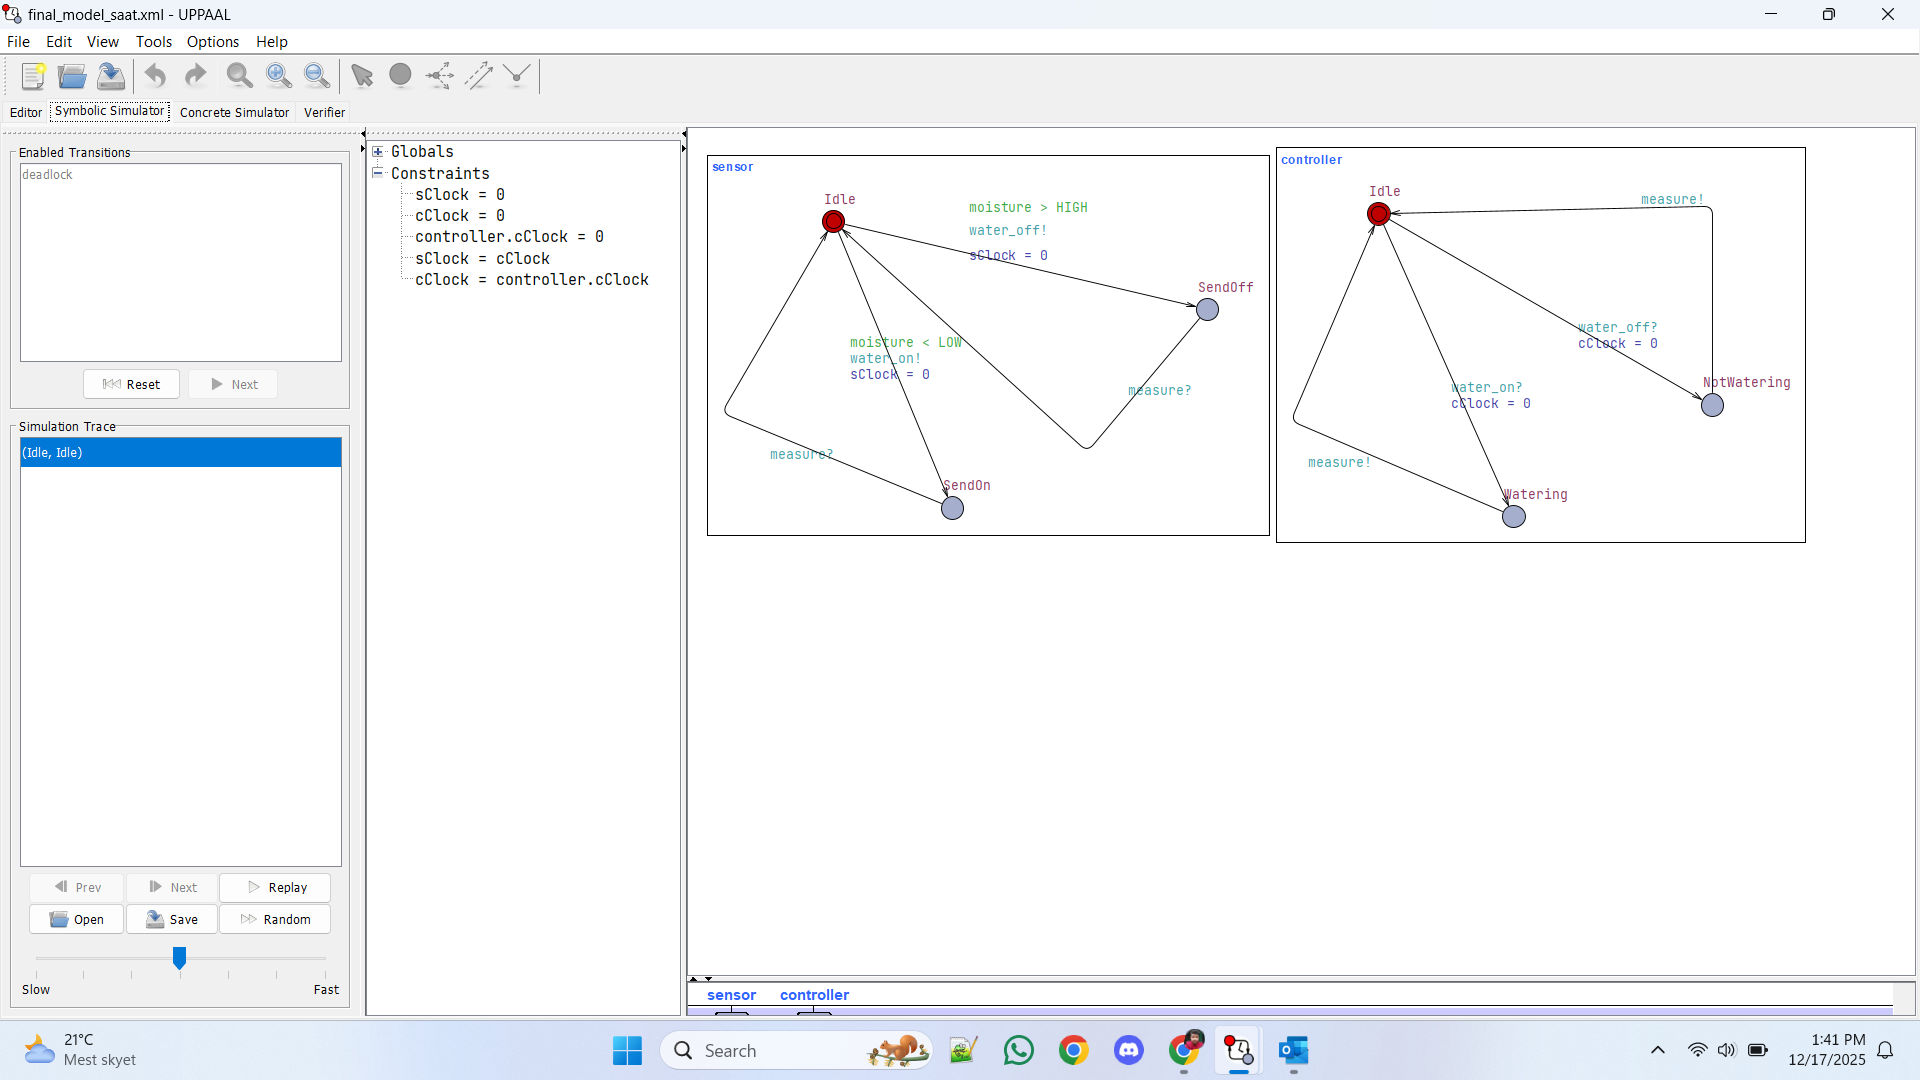
\includegraphics[width=85mm]{uppaal.png}
  \caption{Formal Validation}
  \label{fig:Formal Validation}
\end{figure}

\subsection{Modeling Approach}

A network of two communicating timed automata—a Sensor automaton and a Controller automaton—is used to model the system. In the suggested architecture, these elements illustrate the fundamental relationship between irrigation control and soil moisture monitoring. Synchronous channels are used to enable deterministic and lossless message flow across automata. Two clocks are used in this model.

\begin{itemize}
    \item sClock, associated with the Sensor, to model sensing and reporting intervals;
    \item cClock, associated with the Controller, to model reaction time and watering duration
\end{itemize}

This approach allows both event-based behavior and time constraints to be explicitly analyzed.

\subsection{Sensor Automaton}

The Sensor automaton simulates reporting and measuring soil moisture. It is made up of the following states:

\begin{itemize}
    \item Idle: Soil moisture can now be measured by the sensor.
    \item SendOn: Indicates that low soil moisture (below a predetermined threshold) has been detected.
    \item SendOff: Indicates that high soil moisture (over a predetermined threshold) has been detected.
\end{itemize}

The sensor alerts the Controller with a water\_on! signal when soil moisture falls below the lower threshold. On the other hand, a water\_off! signal is sent when soil moisture surpasses the upper threshold. The sensor waits for a fresh measurement request (measure?) from the Controller after transmitting a signal. Every time a transition occurs, the sensor clock is reset to guarantee that all data are accurate and timely.

\section{Evaluation}
\label{sec:evaluation}

% Empirical evaluation
This Section describes the evaluation of the proposed design.
Section \ref{sec:design} introduces the design of the experiment to evaluate the system. 
Section \ref{sec:measurements} identifies the measurements in the system for the experiment.
Section \ref{sec:pilot_test} describes the pilot test used to compute the number of replication in the actual evaluation. 
Section \ref{sec:analysis} presents the analysis of the results from the experiment. 

\subsection{Experiment design}
\label{sec:design}

To complement the formal analysis, we also evaluated the running system with an experiment. The goal was to see how the architecture behaves under increasing load and if it still fulfills our performance-related QAS.

\begin{itemize}
    \item Independent variable: number of simulated greenhouses (5,10).
    \item Dependent variables:\\
 – number of processed requests within 30 seconds,\\
 – percentage of failed requests.
\end{itemize}

The SimulatorUI sends soil moisture events for each greenhouse at a fixed rate. These events are sent through RabbitMQ to the relevant services, which update the database and the Dashboard. For each configuration we reset the system, start the simulation and measure the metrics over 30 seconds. This follows the general experiment process with scoping, planning, operation, analysis and presentation.

\subsection{Controller Automaton}

The irrigation control logic is modelled by the Controller automaton. It is made up of the following states:

\begin{itemize}
    \item Idle: The controller is awaiting input from the sensor.
    \item Watering: The irrigation system is working.
    \item The irrigation system is inactive.
\end{itemize}

The Controller enters the Watering state and turns on irrigation when it receives a water\_on? signal. It changes to the NotWatering state when it receives a water\_off? signal. The measure! signal is used by the Controller to regularly request new sensor measurements. Timing restrictions on reaction time and irrigation duration are enforced by the controller clock.

\subsection{Measurements}
\label{sec:measurements}

\begin{figure}[htbp]
  \centering
  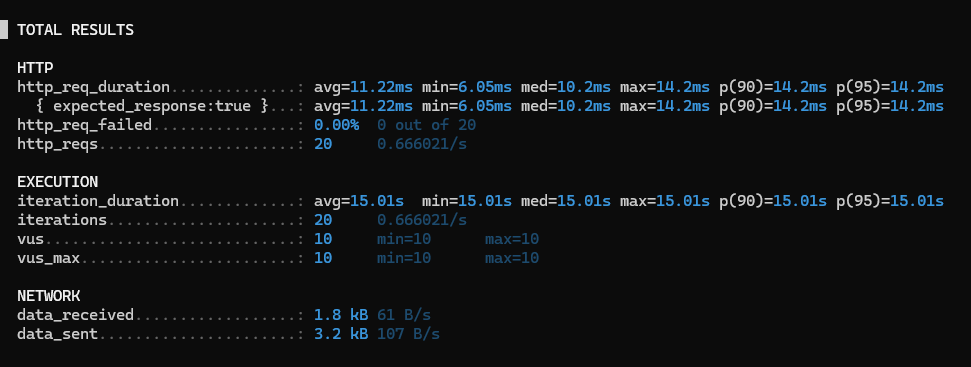
\includegraphics[width=85mm]{measure1.png}
  \caption{Measurement: 1 }
  \label{fig:Measurement: 1}
\end{figure}

\begin{figure}[htbp]
  \centering
  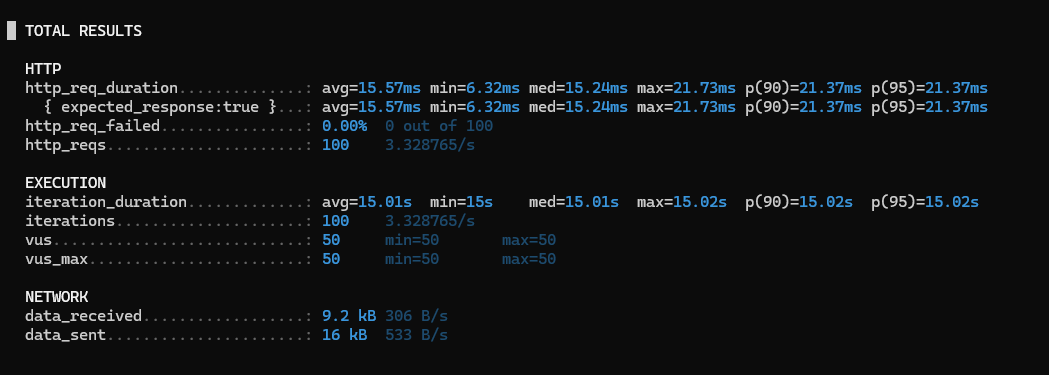
\includegraphics[width=85mm]{measure2.png}
  \caption{Measurement: 2 }
  \label{fig:Measurement: 2}
\end{figure}

\begin{figure}[htbp]
  \centering
  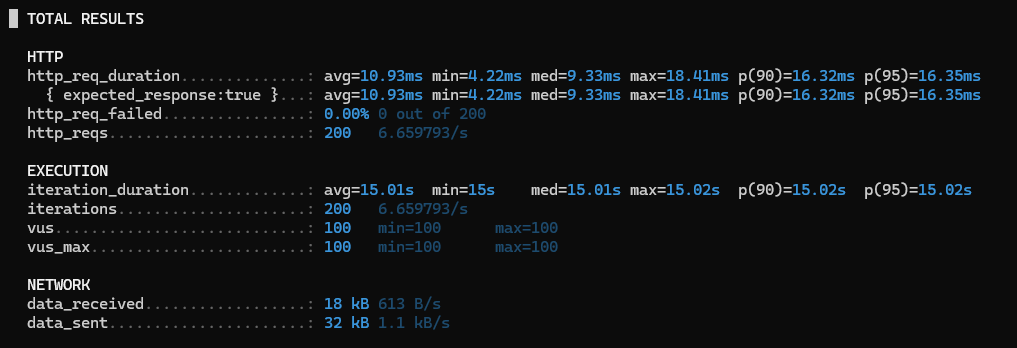
\includegraphics[width=85mm]{measure3.png}
  \caption{Measurement: 3 }
  \label{fig:Measurement: 3}
\end{figure}

\begin{figure}[htbp]
  \centering
  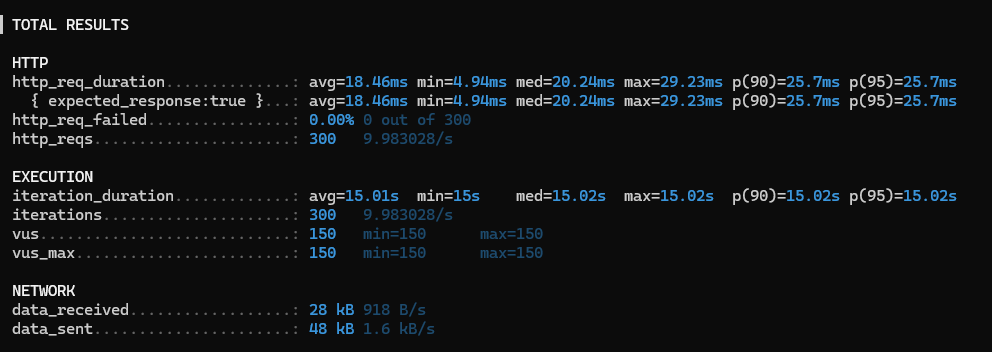
\includegraphics[width=85mm]{measure4.png}
  \caption{Measurement: 4 }
  \label{fig:Measurement: 4}
\end{figure}

\begin{figure}[htbp]
  \centering
  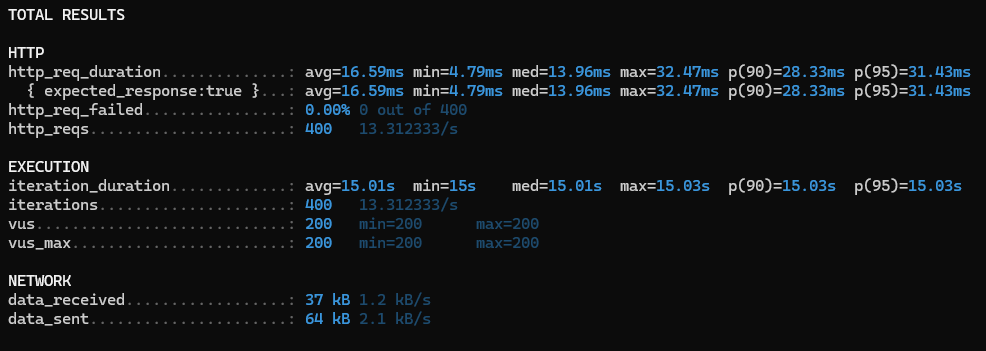
\includegraphics[width=85mm]{measure5.png}
  \caption{Measurement: 5 }
  \label{fig:Measurement: 5}
\end{figure}


\begin{table}[h]
    \centering
    \renewcommand{\arraystretch}{1.2}
    \begin{tabular}{|c|c|c|}
    \hline
        \textbf{Number of Greenhouses} & 
        \textbf{Requests in 30s} & 
        \textbf{Failed Requests (\%)} \\ \hline

        10  & 20  & 0 \\ \hline
        50  & 100 & 0 \\ \hline
        100 & 200 & 0 \\ \hline
        150 & 300 & 0 \\ \hline
        200 & 400 & 0 \\ \hline

\end{tabular}
\caption{System throughput under increasing greenhouse load}
\label{tab:throughput}
\end{table}


\subsection{Pilot test}
\label{sec:pilot_test}

Before we ran all configurations, we did a small pilot test with 3 simulated greenhouses. The purpose was to check if the simulator, RabbitMQ routing and logging worked as expected. During the pilot we discovered some configuration mistakes (e.g. wrong routing key), fixed them, and only then collected the final data. This follows the recommendation from the lectures to use pilot studies to improve the experiment design.


\subsection{Analysis}
\label{sec:analysis}

Based on the results from the measurements in section 8.2 we can conclude that quality attribute number 1 with associated tactics number 1 using RabbitMQ makes it possible to handle high throughput and also makes sure the system can handle higher throughput in the future.


\section{Conclusion}
\label{sec:conclusion}
Conclusion of the report, discussion and relevant future work.

\subsection{Discussion}
\label{sec:Discussion}

In this project we designed, analysed and evaluated a software architecture for a Smart Farming Software Platform that controls multiple greenhouses. We started from use cases and quality attribute scenarios, designed a microservice-based, event-driven architecture with RabbitMQ as middleware, and related our design decisions to architectural tactics and patterns.
Overall, we learned that combining software architecture techniques with formal verification and experiments gives a stronger basis for arguing about system qualities than only looking at code or only looking at diagrams. This is aligned with the course goal of “reasoning about software architecture” and “formal V\&V of software-intensive systems”.


\subsection{Future work}

\label{sec:future_work}

\begin{enumerate}
    \item extend the experiments to longer time periods and higher loads,
    \item include fault-injection scenarios (e.g., RabbitMQ or database failures) to test availability and safety,
    \item model more parts of the system in UPPAAL (for example temperature control),
    \item and add more observability features (metrics, tracing) to the architecture to support continuous evaluation.
\end{enumerate}


\vspace{12pt}

\begin{thebibliography}{9}

\bibitem{bass2013}
L.~Bass, P.~Clements, and R.~Kazman,
\textit{Software Architecture in Practice},
3rd~ed.,
Addison-Wesley, Boston, MA, USA, 2013, p.~69.

\bibitem{alsafi2010}
Y.~Alsafi and V.~Vyatkin,
``Ontology-based reconfiguration agent for intelligent mechatronic systems in flexible manufacturing,''
\textit{Robotics and Computer-Integrated Manufacturing},
vol.~26, no.~4, pp.~381--391, 2010.

\bibitem{angione2017}
G.~Angione \textit{et al.},
``Integration and deployment of a distributed and pluggable industrial architecture for the PERFoRM project,''
\textit{Procedia Manufacturing},
vol.~11, pp.~896--904, 2017.

\bibitem{bass2021}
L.~Bass, P.~Clements, and R.~Kazman,
\textit{Software Architecture in Practice},
4th~ed.,
Addison-Wesley, Boston, MA, USA, 2021.

\bibitem{bengtsson1996}
J.~Bengtsson and K.~G.~Larsen,
``UPPAAL -- a tool for automatic verification of real-time systems,''
in \textit{Proc. DIMACS/SYCON Workshop on Verification and Control of Hybrid Systems},
Springer, 1996, pp.~232--243.

\bibitem{bortolini2018}
M.~Bortolini, F.~G.~Galizia, and C.~Mora,
``Reconfigurable manufacturing systems: Literature review and research trend,''
\textit{Journal of Manufacturing Systems},
vol.~49, pp.~93--106, 2018.

\bibitem{koren1999}
Y.~Koren \textit{et al.},
``Reconfigurable manufacturing systems,''
\textit{CIRP Annals},
vol.~48, no.~2, pp.~527--540, 1999.

\bibitem{koren2010}
Y.~Koren and M.~Shpitalni,
``Design of reconfigurable manufacturing systems,''
\textit{Journal of Manufacturing Systems},
vol.~29, no.~4, pp.~130--141, 2010.

\bibitem{leitao2012}
P.~Leit\~ao, J.~Barbosa, and D.~Trentesaux,
``Bio-inspired multi-agent systems for reconfigurable manufacturing systems,''
\textit{Engineering Applications of Artificial Intelligence},
vol.~25, no.~5, pp.~934--944, 2012.

\bibitem{rabbitmq}
RabbitMQ,
``RabbitMQ documentation,''
Available: \url{https://www.rabbitmq.com/docs},
accessed Dec.~3, 2025.

\bibitem{wan2019}
J.~Wan \textit{et al.},
``Reconfigurable smart factory for drug packing in healthcare Industry~4.0,''
\textit{IEEE Trans. Industrial Informatics},
vol.~15, no.~1, pp.~507--516, 2019.


\end{thebibliography}

\newpage
\section*{Contributions}
\begin{tabular}{l|p{0.6\linewidth}}
Jacmi13 & \begin{itemize}
    \item Use cases,
    \item Quality Attribute scenarios
    \item Design and analysis modelling

\end{itemize}\\

faakt25 & \begin{itemize}
    \item Documentation
    \item Report Writing
\end{itemize}  \\
mmiah25 & Report Writing \\
shbin25 & Formal Validation\\

\end{tabular}
\end{document}